\documentclass{article}
\usepackage{graphicx}
\usepackage{hyperref}

\title{Curriculum Vitae}
\author{Keshav Mishra}
\date{October 15, 2024}

\begin{document}
	\maketitle
	\begin{center}
		c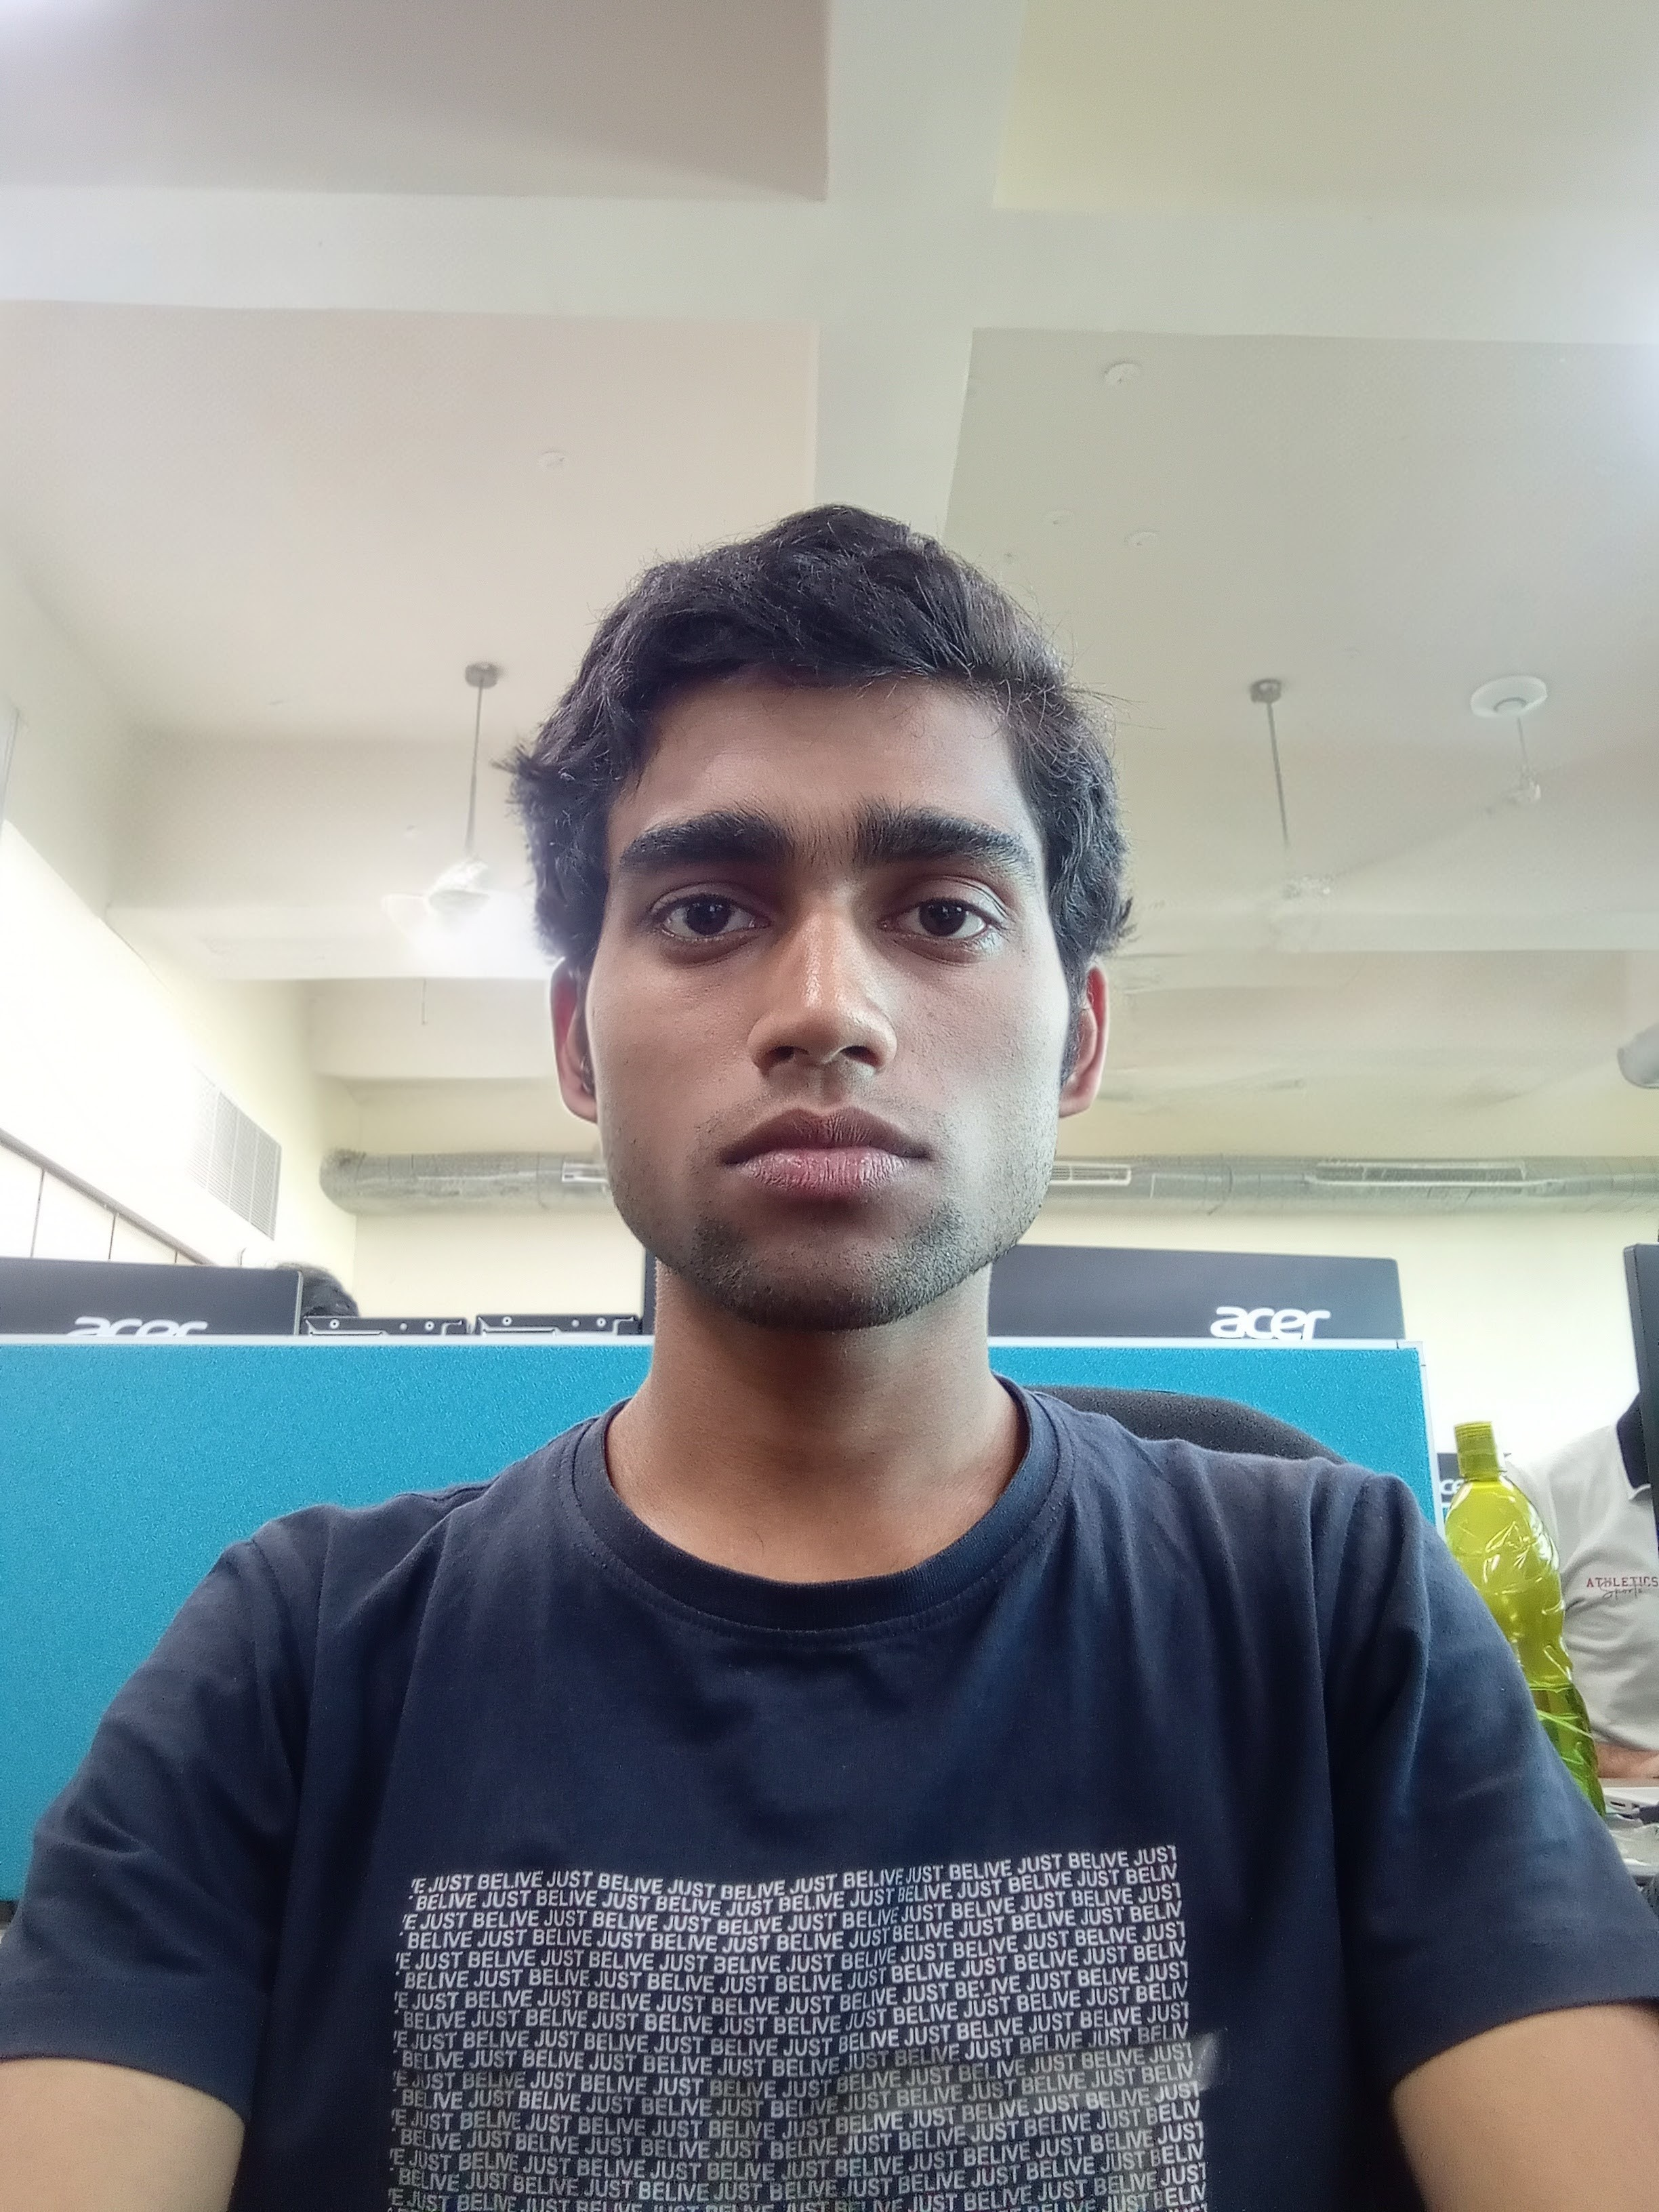
\includegraphics[width=0.3\textwidth]{photo.jpg}
	\end{center}
	\section*{Personal Details}
	\begin{itemize}
		\item Name: Keshav Mishra
		\item Address: Village-Barola, Sec-49, Noida, U.P.
		\item Email ID: \texttt{keshavm@iitbhilai.ac.in}
		\item Contact No: 9717982096
		\item Gender: Male
		\item Date of Birth: December 21, 2004
	\end{itemize}
	
	\section*{Educational Qualifications}
	\begin{tabular}{|c|c|c|c|c|}
		\hline
		\textbf{S.No} & \textbf{Qualification} & \textbf{University} & \textbf{Marks} & \textbf{Year} \\
		\hline
		1 & B.Tech in Computer Science & IIT Bhilai & 9.71 & 2024 \\
		\hline
		2 & 12th & Adarsh Public School & 95.2\% & 2023 \\
		\hline
		3 & 10th & Jesus and Mary Convent School & 91.3\% & 2021 \\
		\hline
	\end{tabular}
	
	\section*{Courses Taken}
	\begin{enumerate}
		\item CS100: Introduction to Programming, Semester I 
		\item PHI102: Physics Lab, Semester I 
		\item MAL100: Mathematics-I, Semester I 
		\item CYL100: Applied Chemistry, Semester I 
		\item PHL101: Physics for Engineers, Semester I 
		\item CYL101: Environmental Science, Semester I 
		\item NCN100: Practices for Comprehension, Semester I 
		\item MEP102: Digital Fabrication, Semester II
		\item EEL101: Basic Electrical Engineering, Semester II
		\item CYP102: Chemistry Lab, Semester II
		\item MAL101: Mathematics-II, Semester II
		\item ECL101: Basic Electronics Engineering, Semester II
		\item BML101: Biology for Engineers, Semester II
		\item LAN103: Professional Ethics, Semester II\\
		
		\href{https://www.iitbhilai.ac.in/index.php?pid=new_schedule_programs}{Courses of Study}
	\end{enumerate}
	
	\section*{Technical Skills}
	\begin{itemize}
		\item Programming Languages: Python, Java, C, C++
		\item Tools: \href{https://www.latex-project.org}{LaTeX}, \href{https://www.visualstudio.com}{Visual Studio}, \href{https://www.github.com}{GitHub}
		\item Frameworks: \href{https://www.djangoproject.com/}{Django}
	\end{itemize}
	
	\section*{Projects}
	\begin{itemize}
		\item Developed an online ticketing website[technologies used: HTML, CSS and JavaScript].
		\item Made a robot car for intra-college competition.
	\end{itemize}
	
	\section*{Extra Curricular Activities}
	\begin{itemize}
		\item I enjoy playing chess, participated in various tournaments.
		\item Participated in Paryatana 2023.
		\item Participated in Inter IIT 2023.
	\end{itemize}
	
	\section*{Other Information}
	\begin{itemize}
		\item I am a Reliance Foundation 2023 Scholar.
	    \item I am a hardworking individual who is passionate about software and computers.
	    \item I strive to give 100\% in everything I do.
    \end{itemize}
	
\end{document}
